\documentclass[a4paper]{article}

%\usepackage{url}

%% Math
\usepackage{mathtools}
%% For Mengen like natural numbers
\usepackage{amsfonts}
%% Für spezielle Symbole
\usepackage{amssymb}

%% Images
\usepackage{import}
\usepackage{xifthen}
\usepackage{pdfpages}
%\usepackage{transparent}

%%% Command for simpler images
\newcommand{\incfig}[1]{%
    \def\svgwidth{\columnwidth}
    \import{./fig/}{#1.pdf_tex}
}

%% Links
\usepackage{hyperref}
\hypersetup{
    colorlinks=true,
    linkcolor=black,
    filecolor=magenta,
    urlcolor=cyan
}

%% Formatting
\usepackage{parskip}
\usepackage{pdflscape}

\title{Datenbanken \\ \large Bäckerei}
\author{Moritz Köhler und Niklas Reusch}

\begin{document}
\maketitle
\tableofcontents
\newpage

% Name der PDF Datei: Bäckereiprojekt_Reusch_Köhler.pdf

% Arbeitszeiten
% 23.09 14:00-16:30
% 24.09 15:15-16:15
% 29.11 21:25-23:15
% 30.11 21:00-22:00
% 03.12 11:10-11:50
% 03.12 13:10-13:30

\section{Anforderungsanalyse}

\begin{flushright}
Moritz Köhler \& Niklas Reusch
\end{flushright}

Um den Überblick über den Verkauf von zahlreichen Produkten einer Bäckerei-Kette zu behalten, müssen diese mit ihrem Produktname, dem zugehörigen Rezept, sowie dem Preis verwaltet werden. Hierbei soll ebenfalls hinterlegt werden, welche Produkte die verschiedenen Filialen der Bäckerei-Kette anbieten und welchen Zutatenbestand diese besitzen. Jede Filiale hat eine eigene Adresse und eine definierte Liste an Zulieferern, von welchen die Zutaten zu einem Festpreis in einer bestimmten Menge gekauft werden.  Da nicht immer in jeder Filiale alle Zutaten des Rezepts zur Produktherstellung vorhanden sind, wird ein Status hinterlegt (z.B. “herstellbar” oder “nicht herstellbar”). Außerdem können die Rezepte eines Produkts je nach Filiale unterschiedlich sein, weshalb es zu den Standard-Rezepten bestimmte Rezept-Varianten gibt. Für spezifischere Abweichungen des Standard-Rezepts soll für die Filialen das Hinzufügen eines Kommentars möglich sein. Zusätzlich hat jede Filiale eigene Mitarbeiter, welche mit ihrem Vornamen, Nachnamen, Adresse, Gehalt sowie dem Geburtsdatum verwaltet werden. Diese sind in bestimmte Schichten eingeteilt, welche zu einem bestimmten Datum und Uhrzeit starten und eine gewisse Dauer haben. Zusätzlich soll ein Überblick über die Verkaufszahlen gewährleistet sein. Hierzu wird eine Verkaufshistorie benötigt, welche zeigt, zu welchem Datum und Menge ein bestimmtes Produkt in einer Filiale verkauft wurde.

\begin{sloppypar}
Außerdem müssen verschiedene Benutzer verwaltet werden, welche unterschiedliche Informationen einsehen und verwalten. Zum einen gibt es die Mitarbeiter einer Filiale, welche ausschließlich Informationen zu den Produkten und Zutatenbeständen der jeweiligen Filiale einsehen und verwalten. Zum anderen gibt es den Filialleiter, welcher alle Informationen zur Filiale einsieht und verwaltet. Diese umfassen nicht nur Produktinformationen, sondern auch Informationen zu den Mitarbeitern, der Kauf- und Verkaufshistorie. Zu guter Letzt gibt es den Eigentümer der Bäckerei-Kette, welcher die Rolle des Administrators einnimmt. Dieser sieht alle Informationen über alle Filialen ein und verwaltet diese.
\end{sloppypar}

\section{ER-Modell}

\begin{flushright}
Niklas Reusch
\end{flushright}

% Wir müssen unsere Anforderungen für das ER Modell so erweitern, dass wir alle möglichen Beziehungen 
% Und wir brauchen ca. 10 Entitäten.

\newpage
\begin{landscape}
    %\begin{figure}[ht]
    %    \centering
    %    \def\svgwidth{\columnwidth}
    %    \import{./fig/}{ERM.pdf_tex}    % Text Scaling done within the .pdf_tex file
    %    \caption{ERM}
    %    \label{fig:ERM}
    %\end{figure}
    \begin{figure}[ht]
        \centering
        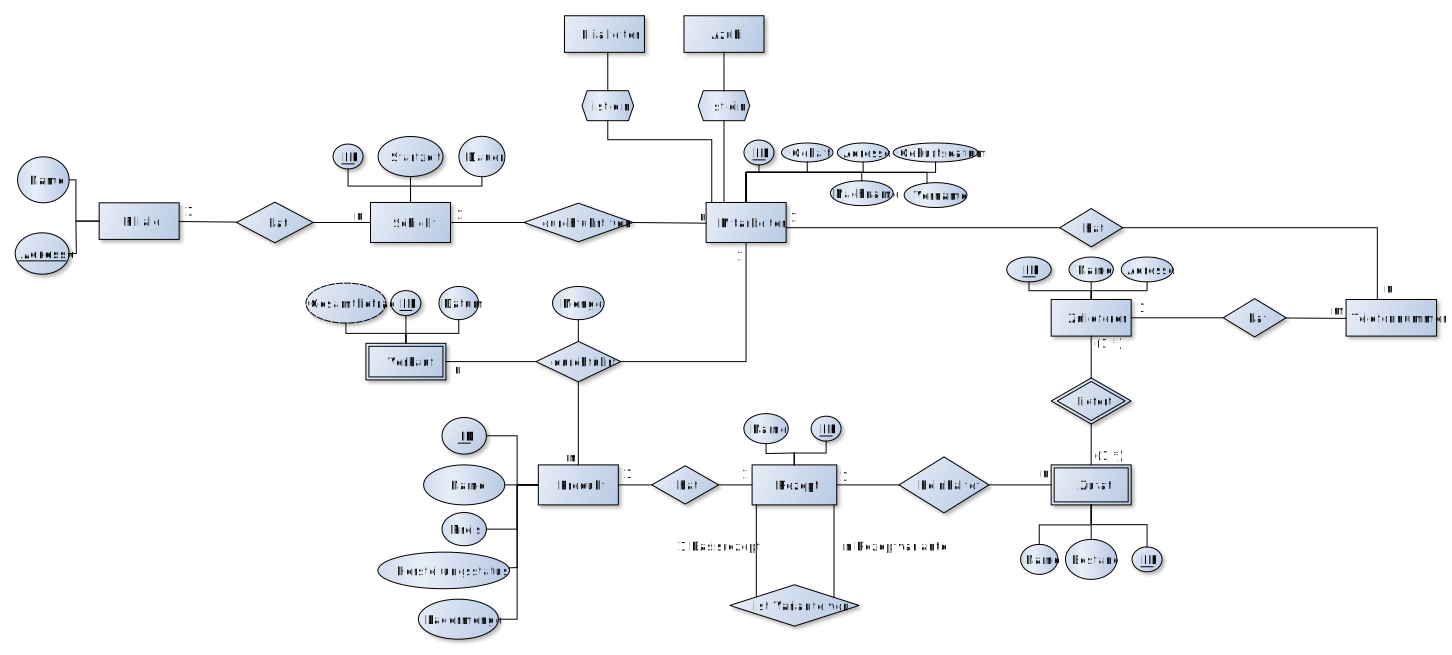
\includegraphics[width=2\textwidth]{./fig/ERM.png}
        \caption{ERM von Niklas Reusch}
        \label{fig:erm_from_niklas_reusch}
\end{figure}
\end{landscape}

\section{Relationale Modell}

\begin{flushright}
Moritz Köhler
\end{flushright}

% Für Normalisierung
% https://normalizer.db.in.tum.de/

% To Do
% Fremdschlüssel hervorheben
% Verkauf fehlt Zuordnung zu Filiale - done
% Produkt, Lagerbestand soll einer Filiale zugeordnet sein - done

\subsection{Entitäten}

Filiale: \{[\underline{FilialeID: integer}, Adresse: string, Name: string, LeiterID: \textit{MitarbeiterID (FS)}]\}

Schicht: \{[\underline{SchichtID: integer}, Startzeit: datetime, Endzeit: datetime, \textit{FilialeID (FS)}: integer]\}

Mitarbeiter: \{[\underline{MitarbeiterID: integer}, Gehalt: integer, Adresse: string, Geburtsdatum: datetime, Nachname: string, Vorname: string]\}

Azubi: \{[\underline{\textit{MitarbeiterID (FS)}: integer}], Start: date, \textit{VerantwortlicherID (FS $\to$ Mitarbeiter)}: integer\}

MitarbeiterTelefonnummer: \{[\underline{Vorwahl: integer, Telefonnummer: integer}, \textit{MitarbeiterID (FS)}: integer]\}

ZuliefererTelefonnummer: \{[\underline{Vorwahl: integer, Telefonnummer: integer}, \textit{ZuliefererID (FS)}: integer]\}

Zulieferer: \{[\underline{ZuliefererID: integer}, Name: string, Adresse: string]\}

% Zutat ist eine Schwache Entität, kann aber von mehreren Zulieferern geliefert werden.
Zutat: \{[\underline{ZutatID: integer, \textit{ZuliefererID (FS)}: integer}, Name: string, Bestand: integer, Einheit: string]\}

% Rekursiv
Rezept: \{[\underline{RezeptID: integer}, Name: string, Anleitung: text, \textit{Basis (FS $\to$ RezeptID)}: integer]\}

Produkt: \{[\underline{ProduktID: integer}, Name: string, Preis: integer, \textit{StatusID (FS)}: integer, Lagerbestand: integer]\}

Verkauf: \{[\underline{VerkaufID: integer}, Datum: datetime, Gesamtbetrag: integer, \textit{FilialeID (FS)}: integer, \textit{MitarbeiterID (FS)}: integer]\}

Status: \{[\underline{StatusID: integer}, name: string, description: string]\}

\subsection{Beziehungen}

durchgeführt-von: \{[\underline{\textit{SchichtID (FS)}: integer, \textit{MitarbeiterID (FS)}: integer}]\}

% beinhaltet: \{[\underline{RezeptID: integer, ZutatID: integer, ZuliefererID: integer}]\}
beinhaltet: \{[\underline{\textit{RezeptID (FS)}: integer, \textit{ZutatID (FS)}: integer}]\}

angeleitet: \{[\underline{\textit{ProduktID (FS)}: integer, \textit{RezeptID (FS)}: integer}]\}

verkauft: \{[\underline{\textit{ProduktID (FS)}: integer, \textit{VerkaufID (FS)}: integer}, Menge: integer]\}

vorhanden: \{[\underline{\textit{ProduktID (FS)}: integer, \textit{FilialeID (FS)}: integer}, \textit{StatusID (FS)}: integer, Lagerbestand: integer]\}

\newpage
\subsection{Normalisierung bis 3NF}

Ausgehend von der großen Relation MVP (Mitarbeiter Verkauft Produkte):

MVP: \{[MitarbeiterID, Gehalt, Adresse, Geburtsdatum, Nachname, Vorname, ProduktID, Produktname, Preis, Status, Lagerbestand, VerkaufID, Datum, Gesamtbetrag, Menge]\}

werden zunächst die funktionalen Abhängigkeiten bestimmt:

\begin{itemize}
    \item MitarbeiterID $\to$ Gehalt, Adresse, Geburtsdatum, Nachname, Vorname.
    \item ProduktID $\to$ Produktname, Preis, Status, Lagerbestand.
    \item VerkaufID $\to$ Datum, Gesamtbetrag.
    \item (VerkaufID, ProduktID) $\to$ Menge.
\end{itemize}

\subsubsection*{Kanonische Überdeckung}

Zur Vorbereitung der 3NF-Synthese wird die Menge der funktionalen Abhängigkeiten in eine kanonische Überdeckung überführt:

\begin{enumerate}
    \item Linksreduktion: Nur die Abhängigkeit mit VerkaufID und ProduktID hat mehrere Attribute auf der linken Seite. Eine Reduktion zeigt, dass beide Attribute notwendig sind. 
    \item Rechtsreduktion: Alle rechten Seiten sind minimal, keine Reduktion notwendig.
    \item Entfernen leerer rechter Seiten: keine vorhanden.
    \item Zusammenfassen von FDs mit identischer linker Seite: nicht erforderlich.
\end{enumerate}

\subsubsection*{Erzeugung der Relationen nach dem Synthesealgorithmus}

Für jede funktionale Abhängigkeit wird eine eigene Relation gebildet:

\begin{enumerate}
    \item Mitarbeiter: \{[\underline{MitarbeiterID}, Gehalt, Adresse, Geburtsdatum, Nachname, Vorname]\}
    \item Produkt: \{[\underline{ProduktID}, Produktname, Preis, Status, Lagerbestand]\}
    \item Verkauf: \{[\underline{VerkaufID}, Datum, Gesamtbetrag, FilialeID, MitarbeiterID]\}
    \item verkauft: \{[\underline{ProduktID, VerkaufID}, Menge]\}
\end{enumerate}

\newpage
\subsubsection*{Überprüfung der Superschlüsselbedingung}

Die Hüllen der Schlüsselattribute werden textuell geprüft:

\begin{itemize}
    \item Hülle von MitarbeiterID: umfasst ausschließlich die Mitarbeiterattribute.
    \item Hülle von ProduktID: umfasst ausschließlich die Produktattribute.
    \item Hülle von VerkaufID: umfasst ausschließlich die Verkaufsattribute.
    \item Hülle von VerkaufID und ProduktID: 
    \begin{itemize}
        \item VerkaufID ergänzt die Verkaufsattribute.
        \item ProduktID ergänzt die Produktattribute.
        \item Kombination ergibt MitarbeiterID und Menge.
        \item Durch die Abhängigkeit von MitarbeiterID werden alle Mitarbeiterattribute ergänzt.
        \item Damit umfasst die Hülle alle Attribute der ursprünglichen Relation.
    \end{itemize}
\end{itemize}

\subsubsection*{3NF-Prüfung der einzelnen Relationen}

Mitarbeiter:

\begin{center}
    \begin{tabular}{l|c|c}
        $X\to\alpha$ & Super Schl. & prim\\
        \hline
        MitarbeiterID $\to$ Gehalt & \checkmark & x \\
        MitarbeiterID $\to$ Adresse & \checkmark & x \\
        MitarbeiterID $\to$ Geburtsdatum & \checkmark & x \\
        MitarbeiterID $\to$ Nachname & \checkmark & x \\
        MitarbeiterID $\to$ Vorname & \checkmark & x \\
    \end{tabular}
\end{center}

Produkt:

\begin{center}
    \begin{tabular}{l|c|c}
        $X\to\alpha$ & Super Schl. & prim\\
        \hline
        ProduktID $\to$ Produktname & \checkmark & x \\
        ProduktID $\to$ Preis & \checkmark & x \\
        ProduktID $\to$ Status & \checkmark & x \\
        ProduktID $\to$ Lagerbestand & \checkmark & x \\
    \end{tabular}
\end{center}

Verkauf:

\begin{center}
    \begin{tabular}{l|c|c}
        $X\to\alpha$ & Super Schl. & prim\\
        \hline
        VerkaufID $\to$ Datum & \checkmark & x \\
        VerkaufID $\to$ Gesamtbetrag & \checkmark & x \\
        VerkaufID $\to$ FilialeID & \checkmark & x \\
        VerkaufID $\to$ MitarbeiterID & \checkmark & x \\
    \end{tabular}
\end{center}

verkauft:

\begin{center}
    \begin{tabular}{l|c|c}
        $X\to\alpha$ & Super Schl. & prim\\
        \hline
        (ProduktID, VerkaufID) $\to$ Menge & \checkmark & x \\
        (ProduktID, VerkaufID) $\to$ MitarbeiterID & \checkmark & x \\
    \end{tabular}
\end{center}

\newpage
\subsubsection*{Schlussfolgerung}

Nach der Zerlegung der ursprünglichen großen Relation in die vier Relationen

\begin{itemize}
    \item Mitarbeiter: \{[\underline{MitarbeiterID}, Gehalt, Adresse, Geburtsdatum, Nachname, Vorname]\}
    \item Produkt: \{[\underline{ProduktID}, Produktname, Preis, Status, Lagerbestand]\}
    \item Verkauf: \{[\underline{VerkaufID}, Datum, Gesamtbetrag]\}
    \item verkauft: \{[\underline{ProduktID, VerkaufID}, Menge, MitarbeiterID]\}
\end{itemize}

konnte für jede Relation durch die 3NF-Prüfung gezeigt werden, dass:

\begin{enumerate}
    \item Die linken Seiten aller funktionalen Abhängigkeiten Superschlüssel der jeweiligen Relation sind.
    \item Die rechten Seiten der Abhängigkeiten aus Nicht-Primattributen bestehen, was in der 3NF erlaubt ist, da die linke Seite jeweils ein Superschlüssel ist.
\end{enumerate}

Daraus folgt, dass alle vier Relationen nun die Bedingungen der 3NF erfüllen. Die ursprüngliche große Relation war dagegen noch nicht in 3NF, da einige funktionale Abhängigkeiten weder einen Superschlüssel auf der linken Seite hatten noch ausschließlich Primattribute auf der rechten Seite. Durch die Zerlegung wurden alle transitive Abhängigkeiten und Verstöße gegen die 3NF beseitigt.

\section{Datenschema in SQL}

\begin{flushright}
Niklas Reusch
\end{flushright}

\section{Entwurf}

\begin{flushright}
Moritz Köhler
\end{flushright}


\newpage
\section{Feedback}

\subsection{Feedback: ER-Modell}

\begin{flushright}
von Moritz Köhler für Niklas Reusch am 16.10.2025
\end{flushright}

Das ERM umfasst schon zum großteil die Anforderungen. Ergänzen kann man noch eine Spezifikation eines Mitarbeiter, den Filialleiter. Dieser leitet dann eine Filiale. Weitere Spezifikationen des Mitarbeiter können sein: Azubi, Besitzer.

Zum Azubi könnte man leicht eine Ternäre Beziehung hinzufügen, die auf der Spezialisierung aufbaut. Ein Mitarbeiter bringt einem Azubi ein Rezept bei.

Des weiteren lassen sich die Beziehungen Filiale führt einen Verkauf durch, Mitarbeiter führt einen Verkauf durch und Ein Verkauf enthält Produkte zu einer Ternäre Beziehung zusammenfassen. Die Attribute von der Entität Verkauf kannst du dann einfach an die Beziehung selbst schreiben.

Da Varianten eines Rezeptes selbst ein Rezept sind würde ich dort eine Rekursive Beziehung verwenden. Damit hätten wir dann auch eine Rekursive Beziehung in unserem ERM.

Ich bin mir bei der Rezept besteht aus Zutaten Beziehung etwas unsicher ob das tatsächlich eine "besteht aus" Beziehung ist.

Allgemein zum Format in yEd. Die Telefonnummer von Mitarbeiter und Zulieferer kann gerne mit nach oben, da diese unten mit den sehr Langen Verbindungen komisch aussieht. Es wäre auch schön, wenn die Abstände und Größen der Entitäten und Beziehungen gleich bleiben.

Bitte benutze für die Attribute auch das Attribut Feld unter dem Tab Entity Relationship statt dem Gelben aus Shapes. Für die Spezifikation kann man ein Sechseck aus BPMN benutzen und die Farben aus einer Entität kopieren. Dann sieht alles Einheitlich aus.

\newpage
\subsection{Feedback: Relationale Modell}

\begin{flushright}
von Niklas Reusch für Moritz Köhler am 30.11.2025
\end{flushright}

Das relationale Datenbankmodell umfasst im Wesentlichen alle Anforderungen. Die Relationen und Entitäten aus dem ERM werden sinnvoll zusammengefasst und korrekt dargestellt. Positiv hervorzuheben ist die Auslagerung der Telefonnummern von Mitarbeitern und Zulieferern in eigene Relationen, da beide Entitäten mehrere Telefonnummern besitzen können. Dies ermöglicht eine eindeutige und saubere Zuordnung der Fremdschlüssel. 

Die Primärschlüssel sind den richtigen Relationen zugeordnet und korrekt markiert. Die Fremdschlüssel befinden sich ebenfalls in den zugehörigen Relationen, werden jedoch nicht explizit als solche gekennzeichnet. Dies ist nicht kritisch, da sie aus den Attributbezeichnungen klar hervorgehen, könnte aber zur besseren Lesbarkeit ergänzt werden. 

Außerdem ist der Relation "Verkauf" keine Filiale zugeordnet, wodurch nicht ersichtlich wird, in welcher Filiale ein Verkauf stattgefunden hat. Zusätzlich besitzt ein Produkt einen globalen Lagerbestand, der nicht mit einer Filiale zusammenhängt. Eine mögliche Lösung wäre, der Relation "Verkauf" eine FilialeID zuzuordnen und den Lagerbestand als eigene Relation zwischen Produkt und Filiale zu führen. 

Die Relationen erfüllen die Anforderungen der dritten Normalform, da alle Nicht-Schlüsselattribute voll funktional von ihren Primärschlüsseln abhängen. 

Die Normalisierung in die dritte Normalform mithilfe des Synthesealgorithmus ist logisch nachvollziehbar. Allerdings wäre eine argumentative Überprüfung der ersten und zweiten Normalform einfacher. Zudem wurde die Überprüfung für mehrere Relationen durchgeführt, was aber nicht notwendig wäre. Insgesamt sind der Entwurf in das relationale Schema, sowie die Normalisierung der Relationen gut gelungen.

% \newpage
\subsection{Feedback: Datenschema}

\begin{flushright}
von Moritz Köhler für Niklas Reusch
\end{flushright}



% \newpage
\subsection{Feedback: Entwurf}

\begin{flushright}
von Niklas Reusch für Moritz Köhler
\end{flushright}



\end{document}